\documentclass{article}
\usepackage[utf8]{inputenc}
\usepackage[margin=1in]{geometry}

\title{Shortest Paths}
\author{Kevin Geng}
\date{28 October 2016}

\usepackage{algorithm}
\usepackage{algorithmicx}
\usepackage[noend]{algpseudocode}

\usepackage{tikz}
\usetikzlibrary{calc,shapes.multipart,chains,arrows,positioning}
\tikzstyle{vertex}=[draw,fill=myseagreen,circle,minimum size=24pt,inner sep=0pt]
\tikzstyle{splitvertex}=[draw,fill=myseagreen,circle split,minimum size=24pt]

\definecolor{myseagreen}{RGB}{240,220,180}


\begin{document}

\maketitle

\section{Introduction}

The shortest-paths problem comes up a lot in competitive programming. Given two nodes $u$ and $v$ in a directed graph, we want to find a path between $u$ and $v$ such that the sum of the edge weights of the path is minimized.

\begin{center}
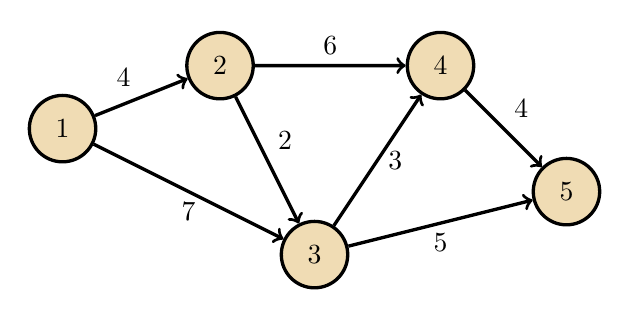
\begin{tikzpicture}[very thick,edge from parent/.style={draw,<-},level/.style={sibling distance=30mm/#1},scale=0.8]
\draw (0, 1) node [vertex] (v1) {1};
\draw (2.5, 2) node [vertex] (v2) {2};
\draw (4, -1) node [vertex] (v3) {3};
\draw (6, 2) node [vertex] (v4) {4};
\draw (8, 0) node [vertex] (v5) {5};
\draw[->] (v1) -- (v2) node[midway, above left] {4};
\draw[->] (v2) -- (v3) node[midway, above right] {2};
\draw[->] (v1) -- (v3) node[midway, below] {7};
\draw[->] (v2) -- (v4) node[midway, above] {6};
\draw[->] (v3) -- (v4) node[midway, right] {3};
\draw[->] (v3) -- (v5) node[midway, below] {5};
\draw[->] (v4) -- (v5) node[midway, above right] {4};
\end{tikzpicture}
\end{center}


\section{Floyd-Warshall}

The Floyd-Warshall algorithm solves the multi-source shortest paths problem; that is, it solves the shortest path problem for every pair of vertices. We use a matrix of distances $dist$, which stores the shortest distance we have found so far for each pair of vertices.

Then, for every vertex $k$, and every pair of vertices $i \rightarrow j$, we try to see if $dist(i,j)$ can be improved by going through $k$. In other words, if the current best distance from $i \rightarrow k \rightarrow j$ is shorter than the current best distance for $i \rightarrow j$ (which could be $\infty$). If it is, we update $dist(i,j)$, which we want to be as short as possible. This is similar to the \textit{relax} operation that we will use for Dijkstra's algorithm, though it may not necessarily involve edges in the original graph.

\begin{algorithm}[H]
\caption{Floyd-Warshall}
\begin{algorithmic}
\State $dist(i, j) \gets \infty$ for vertices $i, j$
\ForAll{vertices $i$}
    \State $dist(i,i) \gets 0$
\EndFor
\ForAll{edges $(u,v)$}
	\State $dist(u,v) \gets weight(u,v)$
\EndFor
\ForAll{vertices $k$}
	\ForAll{vertices $i$}
    	\ForAll{vertices $j$}
        	\If{$dist(i,j) > dist(i,k)+dist(k,j)$}
            	\State $dist(i,j) \gets dist(i,k)+dist(k,j)$
            \EndIf
        \EndFor
    \EndFor
\EndFor
\end{algorithmic}
\end{algorithm}

One way to see why this works is to consider two vertices $u$ and $v$ for which we already know the shortest path from $u \rightarrow v$. Once we consider each of the vertices in that shortest path, $dist(u,v)$ will be the length of the shortest path.


\section{Dijkstra's algorithm}

Those of you who have already taken AP Computer Science should already be familiar with Dijkstra's algorithm, so we won't spend too much time explaining the algorithm itself.

Dijkstra's algorithm calculates the shortest path from a source vertex $u$ to every other node in the graph. If we're only interested in the shortest path from $u \rightarrow v$, we can stop once we remove $v$ from the priority queue.

But why does it work? Every time we remove a vertex $u$ from $pq$, $dist(u)$ is monotonically increasing. This is because the priority queue always gives the minimum element, and for any $u$ removed from the priority queue with neighbor $v$ added to it, $dist(v) < dist(u)$.

\begin{algorithm}[H]
\caption{Dijkstra's algorithm}
\begin{algorithmic}

\ForAll{vertices $v$}
    \State $dist(v) \gets \infty$
    \State $prev(v) \gets -1$
    \State $visited(v) \gets false$
\EndFor

\State $dist(src) \gets 0$
\State $pq \gets$ priority queue
\State add $src$ to $pq$ with key $0$

\While{$pq$ is not empty}
    \State $u \gets u$ in $pq$ with minimum $dist(u)$
    
    \If{$visited(v)$}
    \Comment{only remove each node once}
        \State \textbf{continue}
    \EndIf
    \State $visited(v) \gets true$

    \ForAll{neighbors $v$ of $u$}
    \Comment{relax edges}
        %\If{$visited(v)$}
        %    \State \textbf{continue}
        %\EndIf
        \State $alt \gets dist(u) + weight(u, v)$
        \If{not $visited(v)$ \textbf{and} $alt < dist(v)$}
            \State $dist(v) \gets alt$
            \State $prev(v) \gets u$
            \State add $v$ to $pq$ with key $dist(v)$
            \Comment add instead of update-key
        \EndIf
    \EndFor
\EndWhile

\end{algorithmic}
\end{algorithm}

An important implementation note: C++ implements a \textbf{max heap} rather than a min heap. You can get around this by negating the values of $dist$, or by using \verb|std::greater| as the comparator.


\subsection{Complexity}

Suppose edge $e$ connects vertices $u$ and $v$. If $dist(v) > dist(u) + weight(e)$, then we define the process of \textit{relaxing} an edge $e$ as $dist(v) \gets dist(u) + weight(e)$.

In the worst case, the algorithm will check every edge, and every edge will be relaxed. Each relaxation requires a priority queue insertion operation of complexity $O(\log V)$. Therefore, the complexity of Djikstra's Algorithm is $O(E \log V)$.


\subsection{Update-key}

When relaxing an edge $u \rightarrow v$, we update the value of $dist(v)$. However, if $v$ is already in the priority queue, this might cause problems: most priority queues do not implement the \textit{update-key} operation in $O(\log{n})$ time.\footnote{You can do this with your own priority queue if you keep a map of key to position in the heap.} Instead, we can simply insert the same vertex into the priority queue with an updated key. The vertex with the lowest key will be the first to leave the priority queue. Then, if we mark that vertex as visited, we can avoid processing it again later.

This increases the maximum size of the priority queue from $V$ to $E$, changing the complexity to $O(E log E)$. In practice, though, this is unimportant as $\log_2 E < 2 \log_2 V$ and the priority queue rarely reaches that size.


\subsection{Extensions}

The idea behind Dijkstra's algorithm can be used to implement other algorithms as well.

\begin{itemize}
    \item In a graph where all edge weights are the same, the priority queue in Dijkstra's algorithm can be replaced by a queue, giving a \textbf{breadth-first search}.

    \item If we are only looking for the shortest path to a destination $dest$, then we can use $dist(v)+h(v,dest)$ as the priority queue key for vertex $v$. This is known as the \textbf{A* algorithm}. This requires a heuristic function $h(u,v)$ that provides a lower bound on $dist(u,v)$; Dijkstra's algorithm simply uses $h(u,v)=0$.

    \item \textbf{Prim's algorithm} for finding the minimum spanning tree of a graph is remarkably similar to Dijkstra's. The only difference is that the graph must be undirected, and we use $weight(u,v)$ instead of $dist(v)$ as the priority queue key. In other words, instead of using the distance to $src$, we use the distance to the tree of vertices in $visited$.
\end{itemize}


\section{Bellman-Ford}
If a graph contains negative edge weights, Dijkstra's algorithm cannot be used, because it is a greedy algorithm. Instead, we can use the \textbf{Bellman-Ford} algorithm, which simply relaxes all $E$ edges, $V-1$ times, which is the maximum path length.

If the graph contains a negative cycle, there is no "shortest" path. However, the Bellman-Ford algorithm is useful for detecting such negative cycles. To do this, we check if any distance needs to be updated after running the loop $V-1$ times. If so, there is a path of length $V$, which is impossible without a negative cycle.

\begin{algorithm}[H]
\caption{Bellman-Ford}
\begin{algorithmic}
\ForAll{vertices $v$}
	\State $dist(v) \gets \infty$
    \State $prev(v) \gets -1$
\EndFor
\State $dist(src) \gets 0$
\For{$i = 1,V-1$}
	\ForAll{edges $(u,v)$}
    \Comment{relax every edge}
		\If{$dist(u)+weight(u,v) < dist(v)$}
    	    \State $dist(v) \gets dist(u)+weight(u,v)$
	        \State $prev(v) \gets u$
        \EndIf
	\EndFor
\EndFor
\ForAll{edges $(u,v)$}
	\Comment{check for negative cycles}
	\If{$dist(u)+weight(u,v) < dist(v)$}
   	    \State{negative cycle detected}
	\EndIf
\EndFor
\end{algorithmic}
\end{algorithm}

The complexity of such an algorithm is obviously $O(E V)$. This can be improved by maintaining a queue of vertices whose distances were updated. Although the worst-case complexity remains the same, the average number of iterations decreases to $E$. However, checking for negative cycles will instead require us to look for cycles in the shortest-path tree\footnote{Well, if there is a cycle, it's not a tree...} defined by $prev$.


\end{document}
